\Section{Дерево отрезков}{\today}{Девятериков Иван}
\Subsection{Дерево отрезков}

Дерево отрезков (ДО или segment tree) --- это структура данных, которая позволяет за асимптотику $\O(\log n)$ реализовать любые операции, определяемые на множестве, на котором данная операция {\bfассоциативна}, занимает $\O(4n)$ памяти, а ее построение требует $\O(4n)$ времени.

\down
Операция $\otimes$ называется {\bfассоциативной}, если ее результат не зависит от того, в каком порядке ее вычислять, то есть если $(a \otimes b) \otimes c = a \otimes (b \otimes c)$.

\down
ДО — очень гибкая структура, и число задач, решаемых ею, теоретически неограниченно. Она часто используется для уменьшения асимптотики (ускорения программы).

\THE{Операции}


\t{get(l, r)} Получить значение $f$ на множестве элементов $[a_l \ldots a_r]$.

\t{update(pos, val)} Обновить значение на позиции $a_{pos}$.

\t{update(l, r, val)} Обновить множество элементов $[a_l \ldots a_r]$.


\Subsection{Структура}

\begin{tabular}{cm{0.70\textwidth}}
	\begin{minipage}{4cm}
		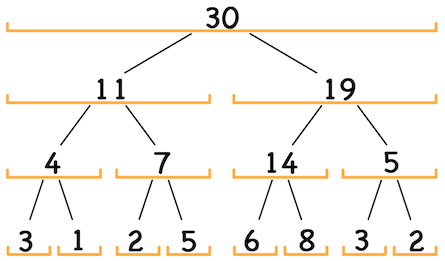
\includegraphics[scale=0.5]{files/sumdo.png}
	\end{minipage} 
	&
Структура представляет собой дерево, листьями которого являются элементы исходного массива. 

Другие вершины этого дерева имеют по два ребенка и содержат результат операции от своих детей (кроме вершин-листьев).

Корень $f(a[0 \ldots n - 1])$, левая $f(a[0 \ldots \dfrac{n}{2}])$, правая $f(a[\dfrac{n}{2} + 1 \ldots n - 1])$ и тд.

Если вершина отвечает за отрезок, то левый и правый сын делят его пополам.
\end{tabular}


\begin{Thm}\label{thm@splay}
ДО хранит в памяти $4n$ вершин (при достраивании до $n=2^k)$.\end{Thm}
\begin{proof}
Понять это можно следующим образом: первый уровень дерева отрезков содержит одну вершину (корень), второй уровень — две вершины, на третьем уровне будет четыре вершины, и так далее, пока число вершин не достигнет $n$. Таким образом, число вершин в худшем случае оценивается суммой 
$1 + 2 + 4 + \dots + 2^{\lceil\log_2 n\rceil} = 2^{\lceil\log_2 n\rceil + 1} < 4n$.
\end{proof}

\begin{Rem}При $n \ne 2^k$, не все уровни дерева отрезков будут полностью заполнены. Например, при $n=3$ левый сын корня есть отрезок $[0 \ldots 1]$, имеющий двух потомков, в то время как правый сын корня — отрезок $[2 \ldots 2]$, являющийся листом. \\
При реализации ДО будем увеличивать его размер до ближайшей степени двойки.
\end{Rem}

\begin{Thm}\label{thm@splay}
Высота ДО $\log n$\end{Thm}
\begin{proof}
Если на одном слое есть $k$ вершин, то на следующем будет $2k$ вершин.
Это следует из количества слагаемых в предыдущем доказательстве.
\end{proof}

\begin{Cons}Время одной операции в ДО -- $\log n$.\end{Cons}

\pagebreak
\up\up\up
\Subsection{Реализация}

ДО можно писать как снизу, так и сверху. Эти подходы лишь различимы по написанию кода, но ДО сверху легче писать и понять. Пока мы будем рассматривать только ДО, написанное {\bfсверху вниз}. Оно представляет собой спуск из вершины в левого и правого сыновей, используя рекурсию. Все запросы будут логично запускаться из корня дерева (самой верхней вершины).

\down
\begin{tabular}{m{0.1\textwidth}m{0.8\textwidth}}
	\begin{minipage}{\textwidth}
\begin{verbatim}
    1  
   / \
  2   3
 / \ / \
4  5 6  7      
\end{verbatim}
	\end{minipage} 
	&
Будем хранить ДО как массив, элементы которого отвечают за результат для текущей вершины в дереве.
Воспользуемся лёгкой формулой для вычисления индексов детей. Если номер корня некоторого поддерева $v$, значит, его левый сын имеет номер $2 \cdot v$, а правый $2 \cdot v + 1$.
\end{tabular}
\down

Такой приём помогает быстрее писать, а также занимает всего $4 \cdot n$ памяти. Это можно заметить, если выписать все номера вершин, они будут образовывать последовательность целых чисел с шагом $1$.

Приёмы, чтобы проще и удобнее писать:

\up \up
\begin{MyList}[0pt]
	\item Определиться с нейтральным элементом --- такой элемент, который не надо рассматривать. Он будет находиться на позициях, в которых нет данных. В ДО на сумму для удобства можно использовать $0$, как нейтральный элемент.
	\item Написать {\bf всего один} раз функцию \t{combine(a, b)}, которая будет принимать два аргумента (результат левого и правого сына) и возвращать результат, который будет записан в корне. И просто вызывать её, когда надо.
	\item Границы запроса использовать не как отрезок, а как полуинтервал $[l, r)$.
	\item Писать всё в одном стиле с одинаковыми переменными, потому что все функции очень похожи.
\end{MyList} \up \up

\THE{Введём обозначения}.

$v$ --- корень некоторого поддерева.

Вершина $v$ отвечает за полуинтервал $[tl, tr)$.

Запросы к ДО будут $[ql, qr)$.

Тогда отрезок, за который отвечает левый сын, будет $[tl, (tl + tr) / 2)]$, а правый --- $[(tl + tr) / 2, tr)$.

Условие, при котором мы будем находиться в листе, когда полуинтервал будет отвечать всего за $1$ элемент, $tl + 1 = tr$.


\pagebreak

\THE{Построение}

Построение --- самая лёгкая функция в ДО. 

Мы спускаемся от корня, идём в сыновья, пока не дойдём до листьев. В лист мы записываем результат, который должен храниться, допустим, это значение в массиве.

Получается, что мы заходим в каждую вершину единожды, а возвращаясь, записываем результат в вершине, равный применению функции \t{combine} от результатов его сыновей. Логично, что в такой рекурсии перед присвоением ответа в вершину, значение в детях будет уже посчитано.
\up \up
\begin{minted}[mathescape,
	linenos,
	numbersep=5pt,
	frame=lines,
	framesep=2mm]{cpp}
void build(int v, int tl, int tr) {
	if (tl + 1 == tr) {
		t[v] = a[tl];
	} else {
		int tm = (tl + tr) / 2;
		build(2 * v, tl, tm);
		build(2 * v + 1, tm);
		t[v] = combine(t[2 * v], t[2 * v + 1]);
	}
}
\end{minted}
\up \up

\THE{Модификация}

\down
\begin{tabular}{cm{0.70\textwidth}}
	\begin{minipage}{4cm}	
		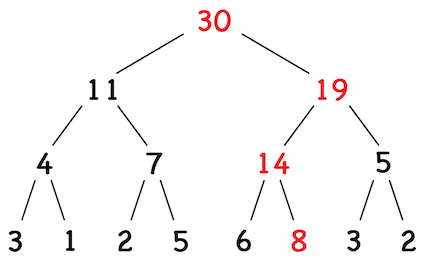
\includegraphics[scale=0.5]{files/set_example.png}
	\end{minipage}
	&
	Когда изменяется элемент массива, нужно изменить соответствующее число в листе ДО, и далее пересчитать значения, которые от этого изменятся.
	
	Надо пересчитать все вершины, которые содержат данный отрезок с этим элементом, заново. Такие вершины лежат по одной на каждом уровне от листа до корня. Значит, их ровно $\log n$.
	
	Находясь в вершине, нам надо спуститься в того сына, который отвечает за отрезок, в котором произойдёт изменение.
\end{tabular}
\down
\up \up
\begin{minted}[mathescape,
	linenos,
	numbersep=5pt,
	frame=lines,
	framesep=2mm]{cpp}
void upd(int v, int tl, int tr, int pos, int val) {
	if (tl + 1 == tr) {
		t[v] = val;
		return ;
	}
	int tm = (tl + tr) / 2;
	if (pos < tm)
	    upd(2 * v, tl, tm, pos, val);
	else
	    upd(2 * v + 1, tm, tr, pos, val);
	t[v] = combine(t[2 * v], t[2 * v + 1]);
}
\end{minted}

\pagebreak

\THE{Запрос получения результата}

Давайте попробуем собрать результат на отрезке $[l \ldots r)$ из уже посчитанных результатов.

Для этого запустим рекурсивный обход дерева отрезков. При этом будем обрывать рекурсию в двух ситуациях.


\begin{MyList}[0pt]
	\item Отрезок, соответствующий текущему узлу не пересекается с отрезком $[l \ldots r)$. В этом случае все элементы в этом поддереве находятся вне области, в которой нам нужно посчитать сумму, поэтому глубже можно не идти.
	\down
	\item Отрезок, соответствующий текущему узлу, целиком вложен в отрезок $[l \ldots r)$. В этом случае все элементы в этом поддереве находятся в области, в которой нам нужно посчитать сумму, поэтому нам нужно добавить к ответу результат этого поддерева, который записан в текущем узле.
\end{MyList}

\begin{center}
	\begin{figure}[h]
		\center{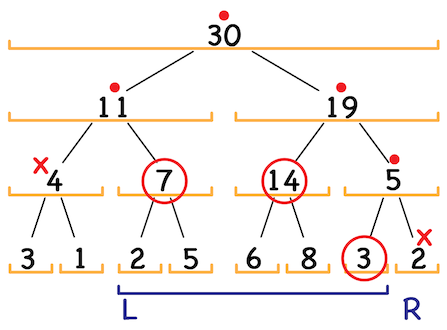
\includegraphics[scale=0.7]{files/get_example.png}}
		\captionsetup{font=small, labelformat=empty}
		\caption{$\times$ - рекурсия оборвалась $\circ$ - число добавилось к ответу, и рекурсия оборвалась}
		\label{fig:image}
	\end{figure}
\end{center}

Чтобы разобраться, почему это работает за $\O(\log n)$, нужно оценить количество «интересных» отрезков --- тех, которые порождают новые вызовы рекурсии. Это будут только те, которые только частично содержат границу запросов — остальные сразу завершатся. Обе границы отрезка содержатся в $\log n$ отрезках, а значит, и итоговая асимптотика будет такая же.

\begin{minted}[mathescape,
	linenos,
	numbersep=5pt,
	frame=lines,
	framesep=2mm]{cpp}
int get(int v, int tl, int tr, int ql, int qr) {
	if (qr <= tl || tr <= ql) {
		ruturn neitral_element;
	}
	if (ql <= tl && tr <= qr) {
		return t[v];
	}
	int tm = (tl + tr) / 2;
	return combine(get(2 * v, tl, tm, ql, qr),
	               get(2 * v + 1, tm, tr, ql, qr));
}
\end{minted}

\pagebreak

\Subsection{Отрезок с максимальной суммой} \href{https://codeforces.com/edu/course/2/lesson/4/2/practice/contest/273278/problem/A}{Задача}

Рассмотрим отрезок $x$, который разделяется на две половинки. Мы хотим для отрезка $x$ найти значение $seg$ — сумму на подотрезке с максимальной суммой. Заметим, что зная только $seg1$ и $seg2$ (ответы для половинок), мы не можем получить $seg$, потому что ответ для $x$ может пересекать оба отрезка.
\down

Но в случае пересечения, отрезок ответа состоит из суффикса левой половины и префикса правой половины. 
\down

Давайте на каждом отрезке будем хранить ещё значения $pref$ и $suf$ --- префикс и суффикс с максимальной суммой. Тогда можно посчитать $seg$ следующим образом: $seg=max(seg1,seg2,suf1+pref2)$.

\begin{center}
	\begin{figure}[h]
		\center{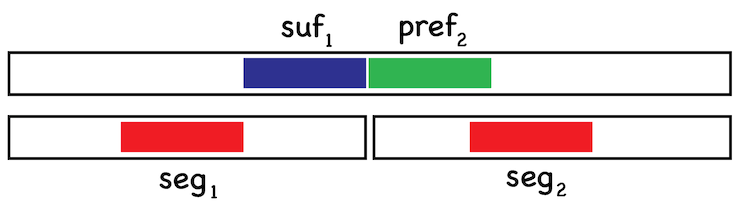
\includegraphics[scale=0.5]{files/max_segment.png}}
	\end{figure}
\end{center}

Пересчёт. Рассмотрим $pref$, $suf$ (будет считаться аналогично).

Для максимальный префикса возможны 2 случая:

\up \up
\begin{MyList}[0pt]
	\item $left_{pref} < len(left_{node})$. Ничего не меняется.
	\item $left_{pref} = len(left_{node})$. Тогда префикс можно дополнить префиксом правой половины.
\end{MyList}
\up \up

Для удобства (чтобы не писать проверки на размеры частей) можно ввести $sum$, равное обычной сумме на отрезке.

Тогда $pref=max(pref1,sum1+pref2)$, аналогично, $suf=max(suf2,sum2+suf1)$.

Если написать \t{combine} аккуратно, то можно будет отвечать на запросы вида $max\_segment(l, r)$. Асимптотика $\O(\log n)$ на запрос.

\Subsection{Максимальная последовательность подряд идущих 0} \href{https://informatics.mccme.ru/mod/statements/view3.php?chapterid=111798}{Задача}

Эта задача похожа на предыдущую. Только тут будем хранить не отрезки для максимальной суммы, а максимальные длины последовательностей из 0. Асимптотика $\O(\log n)$ на запрос.


\Subsection{K-я единица} \href{https://codeforces.com/edu/course/2/lesson/4/2/practice/contest/273278/problem/B}{Задача}

Будем в ДО на сумму хранить только 1, если на данной позиции находится 1, и 0, если иначе.
\down

Нахождение $k$-ой единицы равносильно нахождению самого левого префикса с суммой $k$.

Сумму единиц берём по отрезкам, которые внутри запроса.

Для левой части - $sum(max(l, tl), min(r, tr)))$. Правая часть аналогично.

Если $left_{sum} >= k$, значит, $k$-ая единица находится в левом поддереве, иначе, нам нужно запустить поиск единицы под номером $k - left_{sum}$ в правом поддереве.
\down

Если нет запросов на изменение, для получения количества единиц на отрезке можно использовать префиксные суммы, тогда асимптотика будет $\O(\log n)$ на запрос (тут не надо использовать ДО, и это очень похоже на спуск по отрезкам (бинпоиск)). Эта идея нам поможет далее.

При изменениях элементов префиксные суммы нам уже не помогут. Можно будет использовать ДО, чтобы получать количество $1$ на отрезке (нужные нам для спуска). Тогда асимптотика $\O(\ log ^ 2 n)$ на запросы. 


\begin{tabular}{cm{0.70\textwidth}}
	\begin{minipage}{4cm}
		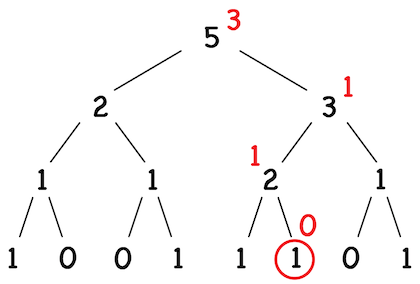
\includegraphics[scale=0.5]{files/k-th.png}
	\end{minipage} 
	&
	Пример запроса \t{find(k=3, [1, 7))}. Мы начинаем в корне, отрезок $[0,8)$. Смотрим на левый подотрезок $[0, 4)$, на нём сумма $sum [1,4) < k$. 
	
	Поэтому мы спускаемся в правый подотрезок $[4,8)$ и ищем на нём $k-sum [1, 4) = 2$-ю единицу. В левом подотрезке $[4,6)$ сумма $sum [4, 6) \ge k$, значит, наша единица лежит в подотрезке $[4,6)$. И наконец, в левом подотрезке $[4,5)$ сумма $1 < 2$, значит, наша единица находится в правом подотрезке $[5,6)$. Ответ $5$.
\end{tabular}

 
\Subsection{Возрастающая на 1 последовательность} \href{https://informatics.mccme.ru/mod/statements/view.php?chapterid=113632}{Задача}

Для удобства сделаем $a_i = a_{i - 1} - 1$.

Данная задача свелась к задаче нахождения максимальной последовательности подряд идущих $0$. Это мы уже умеем делать.

С запросами изменения на отрезке просто. Когда к отрезку добавляется некоторый $x$, это означает, что ответ для отрезка не поменялся. Но поменяться должны элементы на границах, потому что $a_l = a_{l - 1} - 1$ и $a_{r + 1} = a_r - 1$. Тогда надо просто изменить значение в позициях $l$ и $r + 1$. Асимптотика $\O(\log n)$ на запрос.


\Subsection{Посчитать количество и сумму делителей у произведения}

Пусть мы разложим произведение на простые множители $n = p_1^{k_1} \cdot \ldots \cdot p_i^{k_i}$

Количество ($\tau$) и сумма ($\sigma$) делителей --- {\bf мультипликативные функции}.

{\bf Мультипликативные функции} $f(ab) = f(a) \cdot f(b)$ (если $a$ и $b$ {\bf взаимно простые}). 

Пусть $p$ --- простое число.

$\tau(p) = 2 \SO \tau(p^k) = k + 1$ \\
$\tau(n) = (k_1+1) (k_2+1) \ldots (k_i+1)$ \\
$\sigma(p ^ k) = p^0 + p^1 + \ldots + p^k = \frac{p^(k + 1) - 1}{p - 1}$ (геометрическая прогрессия) \\
$\sigma(n) = \sigma(p_1^{k_1}) \cdot \ldots \cdot \sigma(p_i^{k_i})$

\down

В вершине будем хранить разложение на простые множители с их степенями (факторизация). (\t{vector<pair<int, int>>})

Функция \t{combine(a, b)} сольёт два массива в 1 (для одинаковых простых делителей увеличим их степени).

\THE{Асимптотика}

$tau(n)$ и $sigma(n)$ за $\O(len)$ для произвольного $n$.

\t{combine(a, b)} за $\O(len)$

\t{update} будет за $\O(\sqrt x + \log(n) \cdot len)$ 

\t{get} будет за за $\O(\log n \cdot len + len) = \O(\log n \cdot len)$



\Subsection{Ближайший меньший на отрезке}

{\it Решение \NO{1}} За $\log^2 n$

Будем изменять размер отрезка, который будем рассматривать (с помощью простейшего бинпоиска).

Рассмотрим полуинтервалы $[l, m)$ и $[r, m)$, возьмем минимум в них с помощью ДО.

Если в первом полуинтервале есть число $< x$, то мы сдвигаем правую границу, иначе --- левую.

Если ни в первом, ни во втором нет чисел $< x$, тогда ответ не существует.

\down

{\it Решение \NO{2}} За $\log n$

\href{https://codeforces.com/blog/entry/70625}{Обычное ДО на минимум.}

Давайте смотреть на вершины слева направо и делать вот что: если интервал, за который в ДО отвечает левый сын, пересекается с интервалом, на котором мы ищем ответ и минимум в левом поддереве $<x$, то пойдем в левого сына. Если ответ не был найден в левом сыне, то повторим то же самое с правым.

Если левый и правый сын нам не подходят, то перестанем дальше спускаться в эти поддеревьях.

\begin{Thm}\label{thm@splay}
Данная рекурсивная функция займет у нас $\O(\log n)$ времени.
\end{Thm}

\begin{proof}
Пусть мы посетили хотя бы 3 листа. Лист, выходящий за пределы слева и выходящий за пределы справа, и ещё какой-то лист между ними. Если лист с ответом между левой и правой границей, то мы не могли зайти в лист, который за границей справа, потому что попросту обходим слева направо, значит, он совпадает с каким-то из прошлых двух, чего быть не может, ибо мы посещаем каждую вершину по одному разу.

Из того, что мы посетим не более двух листов, очевидно, следует, что асимптотика такого решения $\O(\log n)$.
\end{proof}


\Subsection{Ксюша и битовые операции}

\href{https://codeforces.com/contest/339/problem/D}{Задача}
\href{https://codeforces.com/contest/339/submission/105829607}{\green{AC}}

Рассмотрим получение ответа. Из условия понятно, что она уменьшает длину массива в 2 раза на каждом шаге, только чередуя операцию (побитовое OR/XOR). 

Запишем в дереве на каждом уровне (уровень --- все вершины, которые находятся на одной глубине от корня) результаты операций от двух детей (от соседних следующих элементов), применяя нужную операцию.

\begin{verbatim}
    1         (1): (a1 or a2) xor (a3 or a4) => (2) xor (3)
   / \	       (2): (a1 or a2) 
  2   3       (3): (a3 or a4)
 / \ / \
4  5 6  7      
\end{verbatim}

Эта структура похожа на ДО. Получается, что при в реализации функций \t{build} и \t{update} надо дополнительно поддерживать глубину.

Асимптотика: каждый запрос обновления будет выполняться за $\O(n)$ (массив $a$ размера $2^n$). Памяти при этом требуется $\O(2n)$.

\pagebreak

\Subsection{Сбалансированный плейлист}

\href{https://codeforces.com/problemset/problem/1237/D}{Задача}

Чтобы сделать циклический плейлист линейным, достаточно повторить его три раза.

Для решение данной задачи можно воспользоваться разными подходами. 

{\it Решение \NO{1}} За $O(n \log^2 n)$ или за $\O(n \log n)$, используя разряженную таблицу.

Это идея состоит из 2 частей.
\up \up
\begin{MyList}[0pt]
	\item Используя бинпоиск, будем перебирать границу, когда мы ещё будем слушать.
	\item Проверку отрезка напишем с помощью ДО.
	
	Надо проверить, что $a[pos] > 2 * min(pos, right)$. Здесь $right$ --- правая граница, которую мы рассматриваем, а $pos$ --- первый трек.
\end{MyList}
\up \up
Решение состоит из запросов $min$, бинпоиска, перебора $n$ позиции.

Асимптотика: $O(n \log^2 n)$.
\down

Можно сделать ещё быстрее $min$ за $\O(1)$, если использовать разряженную таблицу.

Асимптотика: $\O(n \log n)$. \href{https://codeforces.com/contest/1237/submission/62698504}{\red{Um\_nik}} \href{https://codeforces.com/contest/1237/submission/63401681}{\red{duality}}

\down

{\it Решение \NO{2}} За $O(n \log n)$ или за $\O(n)$ \href{https://codeforces.com/contest/1237/submission/62704110}{\red{zemen}}

\begin{Prop}Граница, при которой мы закончим слушать, будет не уменьшаться, при сдвиге влево позиции, с которой мы начнём слушать.\end{Prop}

\begin{proof}
	Рассмотрим (правильную) последовательность $a_1, a_2, \ldots, a_x, last$, она обрывается, когда $x=max(a) < \dfrac{last}{2}$. Заметим, что все значения элементов $a$ находятся в $[\ceil[\big]{\dfrac{x}{2}}, x]$. Любые числа из $a$ дают хорошую последовательность.
\end{proof}

Это очень похоже на метод двух указателей c поддержкой максимума $a[i \ldots j]$. Легко написать ДО или использовать метод скользящего окна.

\down

{\it Решение \NO{3}} За $O(n \log n)$
\href{https://codeforces.com/contest/1237/submission/62700019}{\red{300iq}}

Можно решить, сделав поиск ближайшего числа $< \dfrac{x}{2}$, где $x$ --- крутость текущего трека. Это можно сделать с помощью спуска по ДО. Это разбиралось ранее. 

Также можно комбинировать эти идеи.

\href{https://codeforces.com/contest/1237/submission/62700598}{multiset \red{RomaWhite}}

\href{https://codeforces.com/contest/1237/submission/62695687}{map \red{mnbvmar}}

\href{https://codeforces.com/contest/1237/submission/62712896}{st + 2pointer \red{rng\_58}}

\pagebreak

\Section{Дерево отрезков с массовыми операциями}{\today}{Девятериков Иван}
\Subsection{Прибавление на отрезке и значение в точке}

Рассмотрим технику, которая нам пригодится.

\begin{MyList}[0pt]
	\item \t{add(l, r, x)} --- прибавить ко всем $a_i$ $(l \le i \le r)$ значение $x$
	\item \t{get(pos)} --- получить значение $a_i$
\end{MyList}
\up \up

\THE{add}

Чтобы прибавить к элементам на отрезке $[l \ldots r)$ значение $x$, разобьём исходный отрезок на несколько отрезков, каждый из которых покрывается каким-то узлом дерева. Разбиение мы делаем спуском, как до этого.

{\bf Но!} Когда мы находимся в вершине ДО, которая отвечает за отрезок, который внутри запроса обновления, достаточно прибавить к значению в текущем узле $x$.

Время работы операции \t{add} $O(\log n)$ аналогично сумме на отрезке.
\down

Пример вызова: \t{add(3, 8, 5)}
\up \up
\begin{center}
	\begin{figure}[h]
		\center{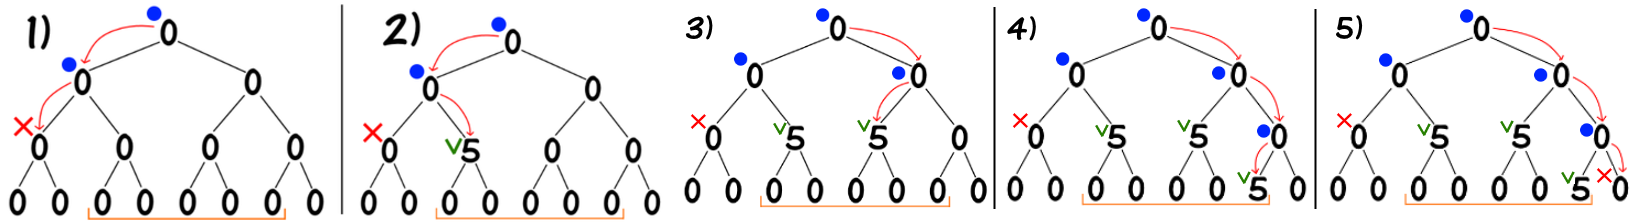
\includegraphics[scale=0.3]{files/AddSegGetPos.png}}
		\captionsetup{font=small, labelformat=empty}
		\caption{$\times$ - рекурсия оборвалась \checkmark - число прибавилось к вершине, и рекурсия оборвалась}
		\label{fig:image}
	\end{figure}
\end{center}

\THE{get}

На значение $a_i$ повлияли только вершины, отрезки которых содержат $i$.

Тогда все изменения, которые могли происходить с данным элементом, находятся на пути от листа до корня. 

Тогда надо просто применить функцию (тут $+$) на пути. Асимптотика $\O(\log n)$ из-за высоты дерева.

\THE{Где это можно использовать?}

Пусть $\otimes$ --- произвольная операция.

Рассмотрим, что будет происходить со значением $a[i]$ при запросах, которые его изменяли. $x$ --- первый запрос, $y$ --- второй.
\down

Спускаясь по дереву от корня до листа, мы пересчитываем значение не в том порядке, как мы их должны были применить, следуя запросам.

$(a[i] \otimes x) \otimes y = a[i] \otimes (x \otimes y)$ --- это ассоциативность.

Также значение $a[i]$ не должно зависеть от порядка запросов над ним.

$a[i] \otimes x \otimes y = a[i] \otimes y \otimes x$ --- это коммутативность.

\THE{Некоммутативные операции}

\begin{tabular}{cm{0.80\textwidth}}
	\begin{minipage}{2.5cm}
		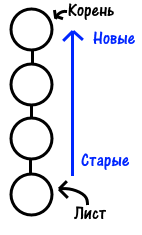
\includegraphics[scale=0.5]{files/AddSegGetPosSort.png}
	\end{minipage} 
	&
	Научимся обрабатывать ассоциативные, некоммутативные операции.
	\down
	
	Будем поддерживать инвариант, что операции на пути от любой вершины дерева до корня отсортированы по времени применения запросов от самых новых до более старых.
\end{tabular}



\begin{tabular}{cm{0.70\textwidth}}
	\begin{minipage}{4cm}	
		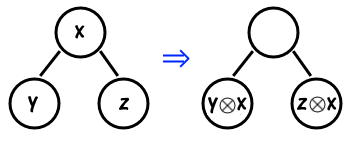
\includegraphics[scale=1.5]{files/AddSegGetPosPush.png}
	\end{minipage} 
	&
	Реализовать это можно с помощью техники проталкивания \t{push}.
	\down
	
	Если в вершине записано значение $x$, а в детях $y$ и $z$, то после проталкивания значение в вершинах будет таким:
	
	\up \up
	\begin{MyList}[0pt]
		\item в левом  $y \otimes x$
		\item в правом $z \otimes x$
		\item в текущей вершине исчезнет $x = -1$ ($-1$ --- пометим, что ничего не надо).
		\down
		
		Мы применили запрос к детям, поэтому текущее значение больше не нужно.
	\end{MyList}
	
	Таким образом, мы сохранили инвариант и освободили текущую вершину.
\end{tabular}

Чтобы применить операцию к некоторой вершине, нужно освободить все вершины на пути от неё до корня, то есть необходимо пройти от корня до вершины сверху вниз и выполнить проталкивания.

Проталкивание работает за $\O(1)$, поэтому мы обрабатываем запросы, как раньше за $\O(\log n)$.

\Subsection{Прибавление и минимум на отрезке}

\begin{MyList}[0pt]
	\item \t{add(l, r, x)} --- прибавить ко всем $a_i$ $(l \le i \le r)$ значение $x$
	\item \t{min(l, r)} --- найти минимум из всех $a_i$ $(l \le i \le r)$
\end{MyList}
\up \up

Давайте использовать два наших подхода. 

Будем в каждой вершине ДО хранить минимум на отрезке и величину, прибавленную на отрезке.

Настоящее значение в вершине --- это минимум в вершине плюс сумма прибавлений от предка этой вершины до корня дерева (изменения только в этих узлах ведёт к изменению текущего минимума). 

$v_{val} = v_{val} + sum(\text{на пути от предка этой вершины до корня дерева })$.
\down


При запросе \t{min(l, r)}, мы будем рекурсивно обходить дерево и поддерживать сумму на пути от корня до предка текущей вершины. 

\pagebreak

Пример: вызова \t{min(4, 7)} после вызова \t{add(3, 8, 2)}

\up \up
\begin{center}
	\begin{figure}[h]
		\center{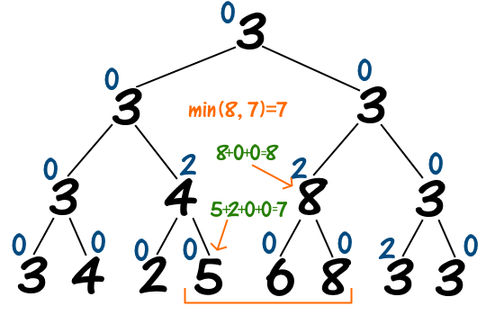
\includegraphics[scale=2]{files/AddSegGetSegMin.png}}
	\end{figure}
\end{center}

Асимптотика $\O(\log n)$.

\THE{Где это можно использовать?}

Пусть у нас есть два вида запросов:

\begin{MyList}[0pt]
	\item \t{modify(l, r, x)} --- применить к каждому $a_i$ $(l \le i \le r)$ $a_i = a_i \otimes x$
	\item \t{calc(l, r)} --- вычислить функцию на отрезке $[l, r]$ $a_l \odot a_{l + 1} \odot \ldots \odot a_r$
\end{MyList}

$\otimes$ и $\odot$ — это любые операции, которые обладают свойствами ниже.
\down

Для вычисления функции на отрезке ($\odot$) надо комбинировать её для детей.

Для изменения на отрезке надо комбинировать старую информацию в узле с новой ($\otimes$).

Следовательно необходимо, \red{чтобы $\otimes$ и $\odot$ были ассоциативными}.
\down

Необходимо, \red{чтобы $\otimes$ была коммутативной}. Для проталкивания.
\down

Мы только что использовали факт, что $min(left + x, right + x) = min(left, right + x)$

Давайте его обобщим:

Мы строим ДО на операции $\odot$.

Тогда результат за который отвечает вершина $v$ будет $v_{val} \otimes x)$.

Но мы знаем что $v_{val} = left \odot right$. Получаем.

Необходимо, $\red{(left \odot right) \otimes x = (left \otimes x) \odot (right \otimes x)}$
\down

Примеры операций, подходящих под условия выше.

\begin{center}
$\begin{array}{| c | c |} \hline \texttt{modify} & \texttt{calc} \\ \hline * & + \\ \hline + & min, max \\ \hline \& & | \\ \hline \end{array}$
\end{center}

Если операция изменения будет сложение, а на заброс сумма. Надо будет сумму на отрезке домножить на его длину.

\pagebreak

\Subsection{Проталкивание}

Это симбиоз всех этих мини-подходов.

Если операция в запросе \t{modify} не коммутативна, то воспользуемся следующей техникой.

Будем сохранять порядок операций, проталкивая старые операции в глубь дерева.

{\bf При любом входе в вершину будем проталкивать} изменение в детей, а при выходе из вершины будем пересчитывать значение от детей.

Пример: прибавление и сумма на отрезке.

\up \up
\begin{minted}[mathescape,
	linenos,
	numbersep=5pt,
	frame=lines,
	framesep=2mm]{cpp}
void push(int v, int tl, int tr) {
    if (tl + 1 == tr) {
        t[v] += lazy[v];
        lazy[v] = 0;
        return ;
    }
    t[v] += lazy[v];
    lazy[2 * v] += lazy[v];
    lazy[2 * v + 1] += lazy[v];
    lazy[v] = 0;
}

void upd(int v, int tl, int tr, int ql, int qr) {
    push(v, tl, tr);
    if (qr <= tl || tr <= ql)  {
        return ;
    }
    if (ql <= tl && tr <= qr) {
        lazy[v]++;
        push(v, tl, tr);
        return ;
    }
    int tm = (tl + tr) / 2;
    upd(2 * v, tl, tm, ql, qr);
    upd(2 * v + 1, tm, tr, ql, qr);
    t[v] = t[2 * v] + t[2 * v + 1];
}
\end{minted}

\pagebreak

\Subsection{Девочка и максимальная сумма}

\href{https://codeforces.com/contest/276/problem/C}{Задача}
\href{https://codeforces.com/contest/276/submission/106207096}{\green{AC}}

Хотя эту задачу можно решить, используя только сортировку. Но мы поступим по-другому. Эти идеи помогут в следующей задаче.

Максимальный ответ можно получить, если мы элементы с большим значением поставим на позиции, в которых происходит больше запросов.

Нам осталось посчитать для каждого индекса количество запросов, которые будут содержать данный индекс. Это можно сделать с помощью прибавления на отрезке (ДО массовое).

После запросов нам надо получить количество в каждом индексе. Можно поступить различными способами. Предлагаю написать вам второй способом.
\down

Способы:

\up \up
\begin{MyList}[0pt]
	\item Для каждой позиции найдём количество, используя функцию $get$.
	
	Асимптотика $\O(m \log n + n \log n))$.
	
	\item  В детях мы содержим не совсем правильную информацию. Она как бы правильная, если учесть массив массовых операций. А что нам мешает последовательно от корня сделать \t{push} от всех вершины? Очень будет похоже на \t{build}, только с \t{push}.
	
\begin{minted}[mathescape,
	linenos,
	numbersep=5pt,
	frame=lines,
	framesep=2mm]{cpp}
void apply(int v, int tl, int tr) {
	push(v, tl, tr);
	if (tl + 1 == tr) {
		return ;
	}
	int tm = (tl + tr) / 2;
	apply(2 * v, tl, tm);
	apply(2 * v + 1, tm, tr);
	t[v] = t[2 * v] + t[2 * v + 1];
}
\end{minted}

	
	После этого все вершины будут хранить правильные ответы. Осталось их получить.
	
	Можно заметить (очень полезный приём), что ответ для $i$-го индекса находится уже на последнем уровне дерева. И мы просто можем получить индекс вершины. Это просто количество вершин на всех уровнях выше плюс $i$. Тогда просто можно сделать цикл.
	
	Асимптотика $\O(m \log n + 4 \cdot n)$.
\end{MyList}

Тут я не учитывал сортировку, так как она незначительно влияет на асимптотику.

\pagebreak

\Subsection{XOR на отрезке}

\href{https://codeforces.com/problemset/problem/242/E}{Задача}

Битовая операция $xor$ {\bfассоциативна}. 

Для чисел в десятичной системе счисления $xor$ применяется как последовательный $xor$ соответствующих разрядов в двоичной системе счисления. Давайте так и сделаем. Запишем все числа в двоичной системе счисления друг под другом. Недостающие разряды дополним $0$. Давайте посмотрим на такую таблицу. 

\down
\begin{tabular}{cm{0.80\textwidth}}
	\begin{minipage}{2.5cm}
		\begin{verbatim}
			100 4    
			1010 10
			11 3
			1101 13
			111 7
			abcd x
		\end{verbatim}
	\end{minipage} 
	&
	Пусть $abcd$ равняется представлению $x$ в двоичной системе счисления.
	
	Тогда $xor$ между битом на некотором разряде со всеми другими битами чисел на отрезке на этом разряде можно сделать ДО (с массовыми) для каждого бита.
	
	Значит, нам надо поддерживать ДО для каждого разряда, а также для этого переписать функции.
	
	\up \up
	\begin{minted}[mathescape,
		linenos,
		numbersep=5pt,
		frame=lines,
		framesep=2mm]{cpp}
void XOR(int ql, int qr, int x) {
	bitset<MAXBIT> ar = x;
	for (int DO = 0; DO < MAXBIT; DO++) {
		upd(DO, 1, 0, MAXN, ql, qr, ar[DO]);
	}
}
	\end{minted}
	\up \up
	
	
	Это легко сделать, если просто добавить вторую размерность: сделать массив дерева вида $t[MAXNBIT][MAXN]$,  а в функцию дополнительно передавать разряд.
	
	Сумму можно получить, последовательно складывая все разряды, домножив их на $2^{\text{в текущем разряде - 1}}$
	
	Количество ДО $MAXBIT=\lceil\log_2 n\rceil = 20$. Асимптотика $\O(20 \cdot \log n)$.
\end{tabular}

\pagebreak

\Subsection{Занятия физкультуры}

\href{https://codeforces.com/contest/915/problem/E}{Задача}
\href{https://codeforces.com/contest/915/submission/106223693}{\green{AC}}

Данную задачу нельзя решить, используя обычное ДО, потому что $n \le 10^9$.

День --- это отрезок длины $1$.

Заметим, что отрезок длины $1$ можно объединить ещё с некоторыми точками рядом, если все текущие сжатые отрезки можно будет сопоставить запросам.

Сопоставление отрезка запросу --- это такой непрерывный отрезок в сжатых отрезках, который явно отвечает за этот вопрос.
\down

Пример отрезков запросов:

$\green{[1, 5]}, \red{[5, 80]}, \yellow{[80, 150]}, \blue{[100, 120]}$

$\green{\Bigg[} 1, \ldots 4, \red{\Big[} 5 \green{\Bigg]}, 6 \ldots 79, \yellow{\Bigg[}80 \red{\Big]}, 81, \ldots, 99, \blue{\Big[}100, \ldots 120 \blue{\Big]}, \ldots 150 \yellow{\Bigg]}$
\down

Пример сжатия:

$\underset{i=1, len = 4}{[1, \ldots 4]}, \underset{i=2, len=1}{[5, 5]}, \underset{i=3, len=74}{[6, 79]}, \underset{i=4, len=1}{[80, 80]}, \underset{i=5, len=19}{[81, 99]}, \underset{i=6, len=21}{[100, 120]}, \underset{i=7, len=30}{[121, 150]}$
\down

Сопоставление запросам:

$\green{[1, 5]} = [1, 4] \cup [5, 5]$

$\red{[5, 80]} = [5, 5] \cup [6, 79] \cup [80, 80]$

$\yellow{[80, 150]} = [80, 80] \cup [81, 99] \cup [100, 120] \cup [121, 150]$

$\blue{[100, 120]} = [100, 120]$
\down


Чтобы обрабатывать общие границы, мы будем добавлять точки $l-1,l,r$.

Тогда мы можем сделать ДО по массиву длин отрезков.

Чтобы понять границы сжатого запроса, достаточно сделать бинпоиск по массиву сжатых границ запросов.

Максимальное количество границ запросов $3 \cdot q$ (это когда все тройки границ для всех элементов различные).

В ДО на сумму надо просто включать/выключать отрезок.

Тогда асимптотика:

\up \up
\begin{MyList}[0pt]
	\item Сортировка тройки границ $\O((3q) \cdot \log 3q)$.
	
	\item Два бинпоиска для получения каждой границы в ДО. $\O(2q \cdot \log 3q)$.
	
	\item Изменение при обработке запроса в ДО. Для каждого запроса $\O(\log 3q)$.
	
	\item Ответ на каждый запрос находится в корне, заранее сделаем от него \t{push}.
\end{MyList}

Итоговая асимптотика $\O((3q) \cdot \log 3q + 2q \cdot \log 3q + q \cdot \log 3q) = \O((3q) \cdot \log 3q) = \O(q \cdot \log q)$.

Также можно решить задачу с помощью динамического ДО.

\Section{codeforces}{\today}{Девятериков Иван}
\Subsection{codeforces}

\href{https://codeforces.com}{codeforces} --- площадка, где регулярно проводятся соревнования.

Плюсы:
\up \up
\begin{MyList}[0pt]
	\item Система с более 6700 официальными задачами (800+ раундов), все задачи готовятся профессионалами.
	\item Много других задач в разделе «Тренировки».
	\item Бесплатно.
	\item Очень быстрые сервера.
	\item Можно посмотреть любое решение любых задач участников.
	\item Можно посмотреть тест (не полностью).
	\item Есть классификация задач. Поиск по типам задач. 
	\item Есть разбор к каждой задаче.
	\item Есть социальная сеть внутри сайта.
	\item Есть система рейтинга.
\end{MyList} \up \up

\Section{Дебаг и cтресс-тестирование}{\today}{Девятериков Иван}
\Subsection{Дебаг}

\up \up
\begin{MyList}[0pt]
	\item Сделать размер массива маленьким. Оптимально $16$ элементов.
	\item Посмотреть, что происходит с запросами и деревом. Попутно нарисовав его на листочке.
	\item Посмотреть тест (или его большую часть).
	\item Написать стресс-тест.
\end{MyList} \up \up

\Subsection{Стресс-тест}

Cтресс-тестирование - это метод, с помощью которого мы можем запустить наше решение (которое, не правильное) на случайных тестах и сопоставить его результат с вывод решения, которое является решением грубой силы (медленное но точно правильное) или принятым решением кого-то другого.

Правильность медленного решения можно проверить, отослав код и оно получает вердикт \red{TL}.

\THE{Требования}:
\up
\begin{MyList}[0pt]
	\item Решение, которое мы хотим протестировать.
	\item Решение методом грубой силы, которое дает правильное решение.
	\item Генератор для генерации тестовых примеров в соответствии с задачей.
\end{MyList} \up \up

\THE{Принцип работы}

\up \up
\begin{MyList}[0pt]
	\item Генерировать случайный тест. Лучше его записать в файл.
	\item Запустить решение, которое даёт правильный ответ но медленно.
	\item Запустить решение, которое неправильное.
	\item Сравнить результаты вывода двух решений.
\end{MyList} \up \up

\THE{Написание отдельного файла для стресс-тестирования}

\up \up
\begin{MyList}[0pt]
	\item Пишите генератор теста и проверку ответов двух решений в одном файле.
	\item Лучше использовать $python$. Получается очень кратко и быстро писать.
	\item Используйте $seed$ для генератора. Чтобы при перезапуске стресс-теста проверять предыдущие тесты. 
\end{MyList}

Есть другой подход в котором мы делаем тоже самое просто внутри основной программы.

Пример стресс-теста в одном отдельном от решения файле на $python$:

\down

\begin{tabular}{cc}
	\begin{minipage}{9cm}
		WA.cpp
		\begin{minted}[mathescape,
			linenos,
			numbersep=5pt,
			frame=lines,
			framesep=2mm]{cpp}
#include <iostream>
int main() {
  int t;
  long long a, b;
  std::cin >> t;
  while (t--) {
    std::cin >> a >> b;
    std::cout << (a + b) % 228 << '\n';
  }
  return 0;
}
		\end{minted}
	\end{minipage} 
	&
	\begin{minipage}{8cm}
		OK.cpp
		\begin{minted}[mathescape,
			linenos,
			numbersep=5pt,
			frame=lines,
			framesep=2mm]{cpp}
#include <iostream>
int main() {
  int t;
  long long a, b;
  std::cin >> t;
  while (t--) {
    std::cin >> a >> b;
    std::cout << (a + b) << '\n';
  }
  return 0;
}
		\end{minted}
	\end{minipage} 
\end{tabular}

\down

\href{https://pastebin.com/cRGvAuPJ}{Код стресса}

\begin{center}
	\begin{figure}[h]
		\center{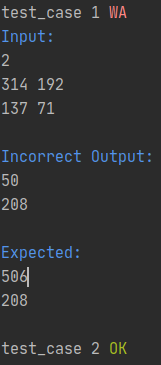
\includegraphics[scale=0.7]{files/stress.png}}
		\captionsetup{font=small, labelformat=empty}
		\caption{Пример вывода}
		\label{fig:image}
	\end{figure}
\end{center}

\Section{Ссылки}{\today}{Девятериков Иван}
\Subsection{Ссылки + задачи, которые будут добавляться}

Простое задание (sort(l, r) string)

Число возрастающих подпоследовательностей DP + DO = $\O(n \ log n)$ (+ которая в Сириусе)

ОКНА

\begin{itemize}
	
	\item \href{https://codeforces.com/blog/entry/22616}{Segment Tree Problems}
	
	\item \href{https://codeforces.com/blog/entry/56880}{Persistent segment tree Problems}
	
	\item \href{https://codeforces.com/blog/entry/55274}{много задач по темам + комментарии}
	
	\item \href{https://codeforces.com}{codeforces} - площадка, где регулярно проводятся соревнования, система с более 6700 официальных задач
	
	\item \href{https://polygon.codeforces.com}{polygon} - сервис для подготовки задач по программированию.
	
	\item \href{https://codeforces.com/blog/entry/83170}{бакалаврская диссертация «Compressed segment trees and merging sets in $O(N \log U)$» } (Lucian Bicsi, Бухарестский университет)
	
	
	\item Книга «Конспект лекций по алгоритмам» (Сергей Копелиович, НИУ ВШЭ)
	
	\item \href{https://codeforces.com/edu/course/2}{Учебный курс} (Павел Маврин, Университет ИТМО)
	\item \href{https://codeforces.com/blog/entry/57319}{A simple introduction to "Segment tree beats"} (Ruyi Ji, Пекинский университет)
	
	\item \href{https://codeforces.com/blog/entry/18051}{Efficient and easy segment trees} (\href{http://finals.snarknews.info/index.cgi?data=2011/teams/knu&class=final2011&year=2011}{Александр Бачериков})
	
	\item \href{https://codeforces.com/blog/entry/15890}{Algorithm Gym :: Everything About Segment Trees} (AmirMohammad Dehghan, Массачусетский технологический институт)
	
	\item \href{https://codeforces.com/blog/entry/80195}{Matrix Exponentiation tutorial} (Kamil Debowski, Варшавский университет)
	
	\item \href{https://codeforces.com/blog/entry/43230}{Mo's Algorithm on Trees} (Animesh Fatehpuria, Технологический институт Джорджии)
	
	\item \href{https://codeforces.com/blog/entry/78898}{Tutorial on Permutation Tree} (Ashley Khoo)
	
	\item \href{https://codeforces.com/blog/entry/61364}{Searching Binary Indexed Tree in $O( \log(N))$ using Binary Lifting} (Siddharth Nayya, Делийский технологический университет)
	
	\item \href{https://e-maxx.ru/algo/segment_tree}{e-maxx.ru/algo/segment\_tree}
	
	\item \href{https://codeforces.com/blog/entry/15729}{много структур}
	
	\item Так же есть Китайскии форумы (я нагуглил китайский аналог статей и там один миоиард китайцев решают задачи с cf) (\href{https://blog.csdn.net/weixin_43826249/article/details/102600666}{Вот пример просто транслейт или учите Китайский})
	
\end{itemize}


\href{https://codeforces.com/blog/entry/49446}{Говорят что это идентичная структура} которая диссертация 

\Subsection{Последние изменения}

Переписана $k$ единица. Написал что можно без изменений префсуммами. Переделал пример (там была поч $k + 1$ единица).

Переписан пример и добавлена картинка в начале реализации ДО.

+ картинки по бокам.

+ дебаг ДО.

+ сделал список из полезных приёмов

+ $max\_sum$

+ $xor$

+ Занятия физкультуры

+ всё о массовых

+ отредактировал везде вёрстку

+ исправил очень много ошибок с русским